\chapter{Beta machine and CPU design}

In this section the different modules making up the beta machine will be studied one by one, from 
their functionality to their design. Simulation results are even provided for some of them. Once the 
different elements are explained, the instruction set desired for the beta machine will be 
described. And finally, the different modules will be connected to each other to form the beta
machine with the desired instruction set.

\section{Beta machine components}

\subsection{Program counter}

The program counter is a module with seven inputs (clk, clk\_en, rst, pcsel, offset, data, pc\_in) 
and two outputs (pc\_out and pc\_next), as shown in Figure \ref{fig:components/pc}. 
Its functions are to provide the current counter on pc\_out ($PC$) and its 
next value ($PC + 4$) on pc\_next, and to react to a control signal named pcsel. This control 
will allow to choose the program counter's operating mode. The different modes and their functions
are listed in Table \ref{tab:pc/modes}. Note that if one connects pc\_new to pc\_in and that pcsel
is set to 0b00, the program counter acts like a simple 32bits counter.

\begin{figure}[H]
    \centering
    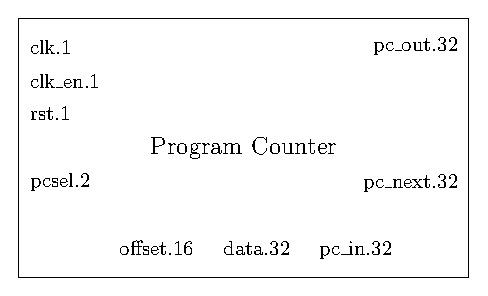
\includegraphics[scale=0.6]{Chapter3-CPU/res/pc}
    \caption{Program Counter}
    \label{fig:components/pc}
\end{figure}

\begin{table}[ht]
    \centering
    \begin{tabular}{|l|l|l|}
    \hline
    \rowcolor[HTML]{DAE8FC} 
    \multicolumn{1}{|c|}{\cellcolor[HTML]{DAE8FC}\textbf{Mode}} & \multicolumn{1}{c|}{\cellcolor[HTML]{DAE8FC}\textbf{pcsel}} & \multicolumn{1}{c|}{\cellcolor[HTML]{DAE8FC}\textbf{Details}}                                                                                                                                                                       \\ \hline
    NORMAL                                                      & 0b00                                                        & \begin{tabular}[c]{@{}l@{}}The current value of the counter program pc\_out becomes \\ the value taken from the input pc\_in.\end{tabular}                                                                                          \\ \hline
    BEQ                                                         & 0b01                                                        & \begin{tabular}[c]{@{}l@{}}The current value of the counter program pc\_out becomes \\ the value taken on the input pc\_in if the value on data is not 0. \\ Otherwise, the current value becomes pc\_in + 4 $\times$ offset.\end{tabular} \\ \hline
    JMP                                                         & 0b10                                                        & \begin{tabular}[c]{@{}l@{}}The current value of the counter program pc\_out becomes the \\ value on data.\end{tabular}                                                                                                              \\ \hline
    BNE                                                         & 0b11                                                        & \begin{tabular}[c]{@{}l@{}}The current value of the counter program pc\_out becomes\\  the value taken on the input pc\_in if the value on data is 0. \\ Otherwise, the current value becomes pc\_in + 4 $\times$ offset.\end{tabular}     \\ \hline
    \end{tabular}
    \caption{Program counter modes}
    \label{tab:pc/modes}
\end{table}

Concerning the internal circuit (that is shown in Figure \ref{fig:components/pc_in}), the pc\_out 
values will be evaluated for the different modes and 
will be put on a multiplexer which will choose the right output according to the pcsel value. For the BNE 
and BEQ modes, another multiplexer is used to make the selection between the two possible results, 
the control of these two multiplexers is naturally done by the result of $data == 0$. 

For the offset, it should be noted that it first undergoes a conversion from 16bits signed to 32bits 
signed before actually being used in the circuit.

The result selected by the multiplexer controlled by pcsel then goes to the register where it is 
stored at the next rising edge of the clock if the clk\_enable is high. The 
pc\_out will thus have the desired value and the pc\_next simply corresponds to pc\_out + 4. When 
the reset (rst) is high, the register is synchronously reset to 0.

\begin{figure}[H]
    \centering
    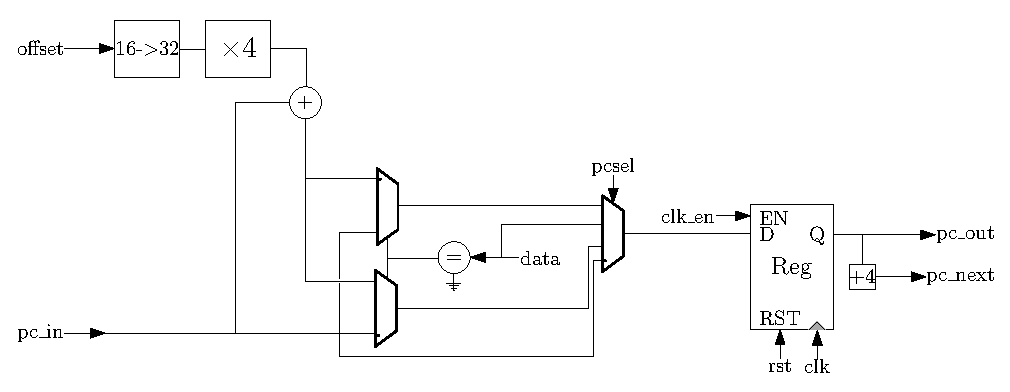
\includegraphics[width=\linewidth]{Chapter3-CPU/res/pc_internal}
    \caption{Program Counter internal circuit}
    \label{fig:components/pc_in}
\end{figure}

\subsubsection*{Program counter simulations}

The different modes of the program counter have been verified by simulation. In the first mode 
(NORMAL mode, pcsel = 0b00), it was checked that with a pc\_in at 4 294 967 292 (the maximum value with 
the last two bits at 0 that helds on 32 bits), the program counter returned 0 for pc\_next and did not 
give a random value. Other random values for pc\_in were checked to be sure that it worked 
correctly. Results of this first simulation are shown in Figure \ref{fig:sim/pc_00}. Note that the
input values are changed only once per two clock cycles but the module is totally able to manage
input changes once per cycle.

\begin{figure}[H]
    \centering
    \includegraphics[scale=0.8]{Chapter3-CPU/res/pc_simu_00.PNG}
    \caption{Program Counter in normal mode simulations for various pc\_in values}
    \label{fig:sim/pc_00}
\end{figure}

To test the JMP mode (pcsel = 0b10), it was simply tried to set data to several values to check if 
pc\_out became this value. Results are provided in Figure \ref{fig:sim/pc_10}.

\begin{figure}[H]
    \centering
    \includegraphics[scale=0.8]{Chapter3-CPU/res/pc_simu_10.PNG}
    \caption{Program Counter in jmp mode simulations for various data values}
    \label{fig:sim/pc_10}
\end{figure}

The last simulation was for the BEQ (pcsel = 01) and BNE (pcsel = 11) modes in order to check 
different offsets (positive and negative) with data fixed at a certain value and then at 0.
Results are given in Figure \ref{fig:sim/pc_01} for BEQ and \ref{fig:sim/pc_11} for BNE.

\begin{figure}[H]
    \centering
    \includegraphics[scale=0.8]{Chapter3-CPU/res/pc_simu_01.PNG}
    \caption{Program Counter in BEQ mode simulations for various data and offset values}
    \label{fig:sim/pc_01}
\end{figure}

\begin{figure}[H]
    \centering
    \includegraphics[scale=0.8]{Chapter3-CPU/res/pc_simu_11.PNG}
    \caption{Program Counter in BNE mode simulations for various data and offset values}
    \label{fig:sim/pc_11}
\end{figure}

In the different simulations the results are all valid, which adds confidence to this design before 
moving on to the practical implementation that will come later.

\subsection{Instruction memory}

\subsection{Register file}

\subsection{ALU}

\begin{figure}[H]
    \centering
    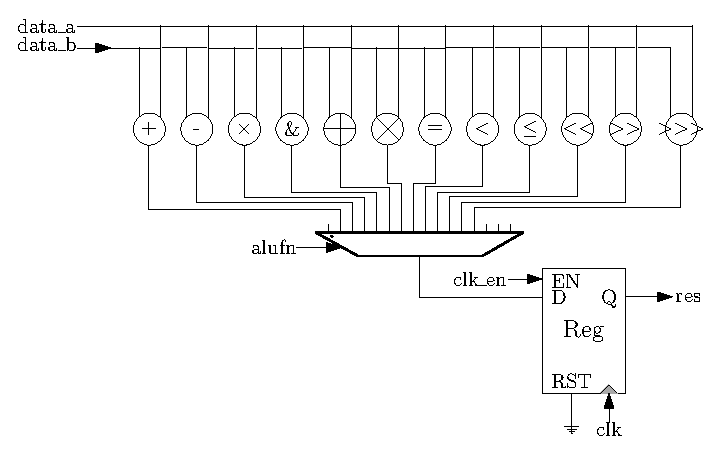
\includegraphics[width=\linewidth]{Chapter3-CPU/res/alu_internal}
    \caption{Arithmetic Logic Unit (ALU) internal circuit}
    \label{fig:components/alu_in}
\end{figure}

\subsection{Data memory}

\subsection{Control logic}

\section{Instruction Set Architecture}
\subsection{Instructions formats}

Two instruction formats are used in the instruction set, the first one is used for all instructions 
requiring two operands ($R_a$ and $R_b$ in Figure \ref{fig:instructions/format}) which will be for example 
the case for simple arithmetic instructions. The second format is used for all instructions 
requiring a single operand and a constant. This will be the case for example for conditional jump 
operations. As can be seen in Figure \ref{fig:instructions/format}, the $R_x$ contain register 
addresses. As they are on 5 bits and no bank change operation exists, 32 registers are addressable. 
$R_c$ stores the result of the instruction when a result exists. It should be noted that the 
constants are on 16 bits and signed.

\begin{figure}[H]
    \centering
    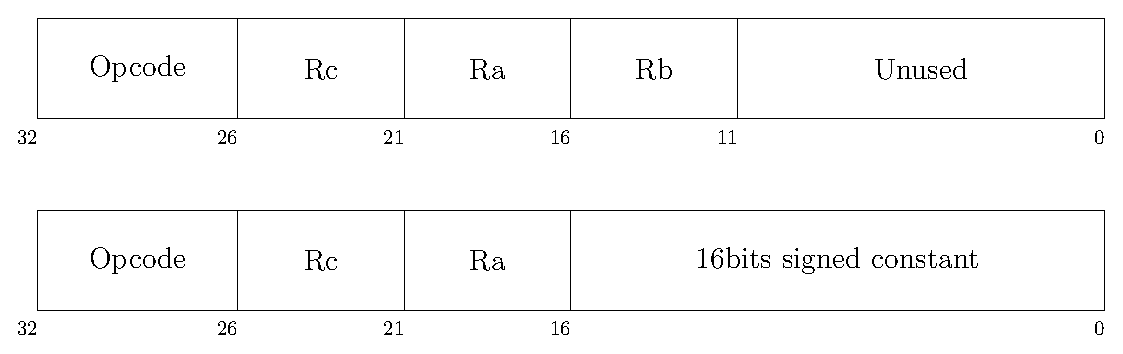
\includegraphics[scale=0.6]{Chapter3-CPU/res/instruction}
    \caption{Instructions format}
    \label{fig:instructions/format}
\end{figure}

\subsection{Instruction set}

\subsubsection*{Arithmetic and logic instructions}

The different arithmetic and logic instructions are managed by the Arithmetic Logic Unit (ALU). The 
different instructions listed in Table \ref{tab:instruction/alu} are supported.

\begin{table}[H]
    \centering
    \begin{tabular}{|l|l|l|l|l|}
    \hline
    \rowcolor[HTML]{DAE8FC} 
    \multicolumn{1}{|c|}{\cellcolor[HTML]{DAE8FC}\textbf{Name}} & \multicolumn{1}{c|}{\cellcolor[HTML]{DAE8FC}\textbf{Operation}} & \multicolumn{1}{c|}{\cellcolor[HTML]{DAE8FC}\textbf{Opcode}} & \multicolumn{1}{c|}{\cellcolor[HTML]{DAE8FC}\textbf{Const Operation}} & \multicolumn{1}{c|}{\cellcolor[HTML]{DAE8FC}\textbf{Const Opcode}} \\ \hline
    Addition                                                    & ADD                                                             & 0x20                                                         & ADDC                                                                  & 0x30                                                               \\ \hline
    Substraction                                                & SUB                                                             & 0x21                                                         & SUBC                                                                  & 0x31                                                               \\ \hline
    Multiplication                                              & MUL                                                             & 0x22                                                         & MULC                                                                  & 0x32                                                               \\ \hline
    Bitwise and                                                 & AND                                                             & 0x28                                                         & ANDC                                                                  & 0x38                                                               \\ \hline
    Bitwise or                                                  & OR                                                              & 0x29                                                         & ORC                                                                   & 0x39                                                               \\ \hline
    Bitwise xor                                                 & XOR                                                             & 0x2A                                                         & XORC                                                                  & 0x3A                                                               \\ \hline
    Compare equal                                               & CMPEQ                                                           & 0x24                                                         & CMPEQC                                                                & 0x3A                                                               \\ \hline
    Compare less                                                & CMPLT                                                           & 0x25                                                         & CMPLTC                                                                & 0x35                                                               \\ \hline
    Compare less or equal                                       & CMPLE                                                           & 0x26                                                         & CMPLEC                                                                & 0x36                                                               \\ \hline
    Logical left shift                                          & SHL                                                             & 0x2C                                                         & SHLC                                                                  & 0x3C                                                               \\ \hline
    Logical right shift                                         & SHR                                                             & 0x2D                                                         & SHRC                                                                  & 0x3D                                                               \\ \hline
    Arithmetic rifht shift                                      & SRA                                                             & 0x2E                                                         & SRAC                                                                  & 0x3E                                                               \\ \hline
    \end{tabular}
    \caption{Arithmetic and logic instructions}
    \label{tab:instruction/alu}
\end{table}

All these instructions simply perform the operation associated with them on the operands $R_a$ and 
$R_b$ in the normal case and on the operands $R_a$ and the constant in the case of instructions 
with constants. $R_a$ will always be used as the first operand. For example, the instruction given 
in Figure \ref{fig:instructions/subc} will result in $[R_{10}] = [R_{14}] - 17$. The notation 
$[R_x]$ means the content of register $R_x$.

\begin{figure}[H]
    \centering
    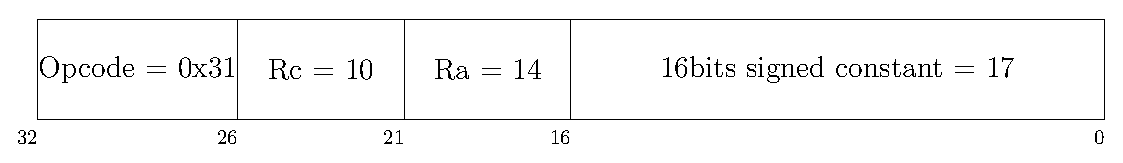
\includegraphics[scale=0.6]{Chapter3-CPU/res/instruction_subc}
    \caption{SUBC instruction example}
    \label{fig:instructions/subc}
\end{figure}

Concerning the comparison operations, they will simply put a $0$ in $R_c$ when the comparison is 
false, a $1$ otherwise.

\subsubsection*{Program counter instructions}

The purpose of these instructions is to modify the value of the program counter conditionally or 
not. The different instructions are listed in Table \ref{tab:instruction/pc}. The values of 
column Next PC will be writen to PC and the address of the next instruction before the jump is
stored in Rc. Note that [Ra] should be byte aligned for JMP but the constant should be 32bits 
aligned for BEQ and BNE (as they already multiply the constant by 4).

\begin{table}[H]
    \centering
    \begin{tabular}{|l|l|l|l|l|}
    \hline
    \rowcolor[HTML]{DAE8FC} 
    \multicolumn{1}{|c|}{\cellcolor[HTML]{DAE8FC}\textbf{Name}} & \multicolumn{1}{c|}{\cellcolor[HTML]{DAE8FC}\textbf{Operation}} & \multicolumn{1}{c|}{\cellcolor[HTML]{DAE8FC}\textbf{Opcode}} & \multicolumn{1}{c|}{\cellcolor[HTML]{DAE8FC}\textbf{Condition}} & \multicolumn{1}{c|}{\cellcolor[HTML]{DAE8FC}\textbf{Next PC}} \\ \hline
    Jump                                                        & JMP                                                             & 0x1B                                                         & None                                                                 & {[}Ra{]} \& 0xFFFFFFC                                         \\ \hline
    Branch Equal                                                & BEQ                                                             & 0x1D                                                         & {[}Ra{]} == 0                                                        & PC + 4 $\times$ (Constant + 1)             \\ \hline
    Branch Not Equal                                            & BNE                                                             & 0x1E                                                         & {[}Ra{]} != 0                                                        & PC + 4 $\times$ (Constant + 1)                \\ \hline
    \end{tabular}
    \caption{Program counter instructions}
    \label{tab:instruction/pc}
\end{table}

\subsubsection*{Memory instructions}

Here, only two instructions are present. One is to load a value from the data memory and the other 
is to store a value in it. The notation $<x>$ means at address $x$ in memory. Note that here $R_c$
doesn't necessarily contains a result at the end of an operation and is used as an operand for ST.
Also, addresses must be byte aligned here and offsets contained in Constant must also be byte
aligned. Both instructions are detailed in Table \ref{tab:instruction/dm}.

\begin{table}[H]
    \centering
    \begin{tabular}{|l|l|l|l|}
    \hline
    \rowcolor[HTML]{DAE8FC} 
    \multicolumn{1}{|c|}{\cellcolor[HTML]{DAE8FC}\textbf{Name}} & \multicolumn{1}{c|}{\cellcolor[HTML]{DAE8FC}\textbf{Operation}} & \multicolumn{1}{c|}{\cellcolor[HTML]{DAE8FC}\textbf{Opcode}} & \multicolumn{1}{c|}{\cellcolor[HTML]{DAE8FC}\textbf{Action}} \\ \hline
    Load                                                        & LD                                                              & 0x18                                                         & {[}Rc{]} = $<${[}Ra{]} + Constant$>$      \\ \hline
    Store                                                       & ST                                                              & 0x19                                                         & $<${[}Ra{]} + Constant$>$ = {[}Rc{]}        \\ \hline
    \end{tabular}
    \caption{Memory instructions}
    \label{tab:instruction/dm}
\end{table}

\subsubsection*{Control instructions}

Only one control instruction exists. This instruction bascally stops the machine and has no operand
or result. The instruction is detailed in Table \ref{tab:instruction/ctrl}

\begin{table}[H]
    \centering
    \begin{tabular}{|l|l|l|}
    \hline
    \rowcolor[HTML]{DAE8FC} 
    \multicolumn{1}{|c|}{\cellcolor[HTML]{DAE8FC}\textbf{Name}} & \multicolumn{1}{c|}{\cellcolor[HTML]{DAE8FC}\textbf{Operation}} & \multicolumn{1}{c|}{\cellcolor[HTML]{DAE8FC}\textbf{Opcode}} \\ \hline
    Exit                                                        & EXIT                                                            & 0x3F                                                         \\ \hline
    \end{tabular}
    \caption{Exit instruction}
    \label{tab:instruction/ctrl}
\end{table}

\section{Beta machine}



\section{CPU design}

